\documentclass[12pt]{amsbook}
\usepackage{preamble}

\newcommand{\vecfieldV}{\boldsymbol{\vec{V}}}
\newcommand{\curvegamma}{\boldsymbol{\vec{\gamma}}}
\newcommand{\tangentgamma}{\boldsymbol{\dot{\vec{\gamma}}}}
\newcommand{\grad}{\boldsymbol{\vec{\nabla}}}
\usepackage{subcaption}
\usepackage{caption}

\renewcommand\thesubfigure{\roman{subfigure}}


\begin{document}
\pagenumbering{gobble}       % This kills the page numbering

\begin{center}
   \textsc{\large MATH 272, Quiz 1}\\
   \textsc{Due February 5$^\textrm{th}$ at the end of class}
\end{center}

\vspace{1cm}

\noindent\textbf{Instructions} \; You are allowed a textbook, homework, notes, worksheets, material on our Canvas page, but no other online resources (including calculators or WolframAlpha) for this quiz.  \textbf{Do not discuss any problem any other person.} All of your solutions should be easily identifiable and supporting work must be shown.  Ambiguous or illegible answers will not be counted as correct.


\vspace*{.5cm}
\hrule
\vspace*{.5cm}

\begin{center}\textbf{\large THERE ARE 6 TOTAL PROBLEMS.}\normalsize \end{center}

\begin{problem}
For the following, describe the domain $D$ and codomain $C$ for the given type of function.
\begin{enumerate}[(a)]
        \item \textbf{(1 pts.)} A curve is a function $\curvegamma \colon D \to C$.
        \item \textbf{(1 pts.)} A scalar field is a function $f \colon D \to C$.
        \item \textbf{(1 pts.)} A vector field is a function $\vecfieldV \colon D \to C$.
\end{enumerate}
\end{problem}

\begin{problem}
    Let $\curvegamma$ be a curve defined by
    \[
    \curvegamma(t) = \begin{pmatrix} e^t \\ e^{-t} \\ t \end{pmatrix} \quad \textrm{for $t\in [0,1]$.}
    \]
    \begin{enumerate}[(a)]
        \item \textbf{(2 pts.)} Compute the tangent vector at time $t$, $\tangentgamma(t)$.
        \item \textbf{(2 pts.)} Compute the speed at time $t$, $\left| \tangentgamma(t) \right|$ (do not feel the need to simplify).
        \item \textbf{(2 pts.)} Let $f(x,y,z) = xyz$. Set up, but do not compute,
        \[
        \int_{\curvegamma} f(\curvegamma) d\curvegamma
        \]
        (do not worry about simplifying this fully).
    \end{enumerate}
\end{problem}

\begin{problem}
    Let $f(x,y,z) = \sin(x)\sin(z)+e^{yz}$.
    \begin{enumerate}[(a)]
        \item \textbf{(2 pts.)} Compute all first order partial derivatives of $f$.
        \item \textbf{(2 pts.)} Compute the laplacian of $f$. 
    \end{enumerate}
\end{problem}

\newpage
\begin{problem}
\textbf{(3 pts.)} Consider the vector field $\vecfieldV$ defined by
    \[
        \vecfieldV(x,y) = \begin{pmatrix} x^2 \\ xy \end{pmatrix}.
    \]
    Plot and label the vector field at the following points.
\begin{enumerate}[i.]
    \item $\vecx_1 = (1,2)$;
    \item $\vecx_2 = (0,-3)$;
    \item $\vecx_3 = (-1,-1)$.
\end{enumerate}
\end{problem}

\begin{problem}
Here is a plot of a 3-dimensional vector field $\vecfieldV$ when viewing from a few different angles.
\begin{figure}[H]
    \centering
    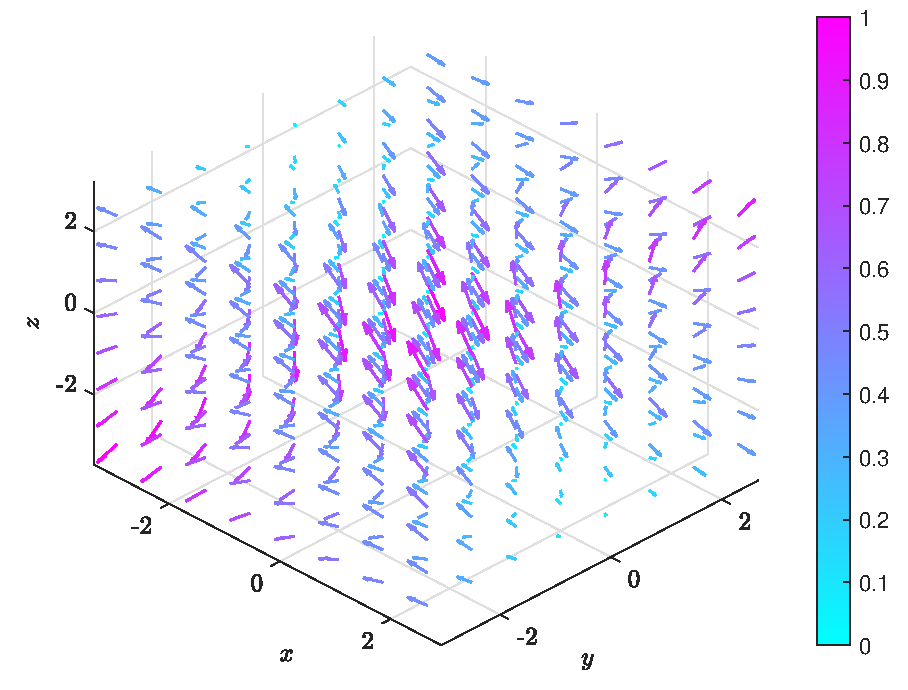
\includegraphics[width=.85\textwidth]{figures/vecfield}
    \caption{A view of the vector field $\vecfieldV$. Note that the colorscaling on this plot represents the length of the vectors. The next plots use the same colorscale.}
\end{figure}
\begin{figure}[H]
    \centering
    \begin{subfigure}[b]{0.45\textwidth}
        \centering
        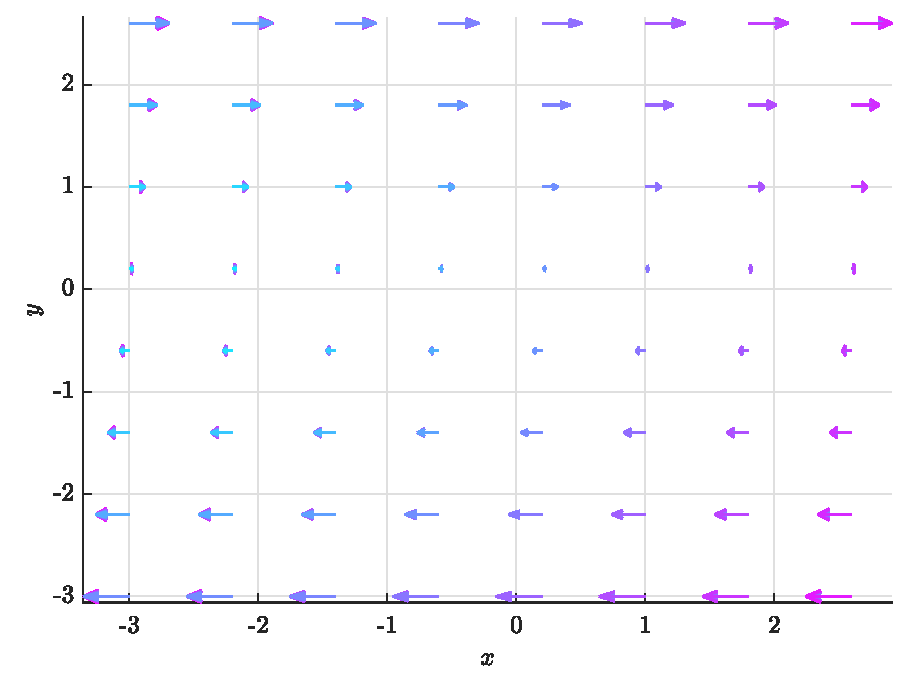
\includegraphics[width=\textwidth]{figures/vecfield_xy}
        \caption{$\vecfieldV$ when looking towards the $xy$-plane.}
    \end{subfigure}
    \quad
    \begin{subfigure}[b]{0.45\textwidth}
        \centering
        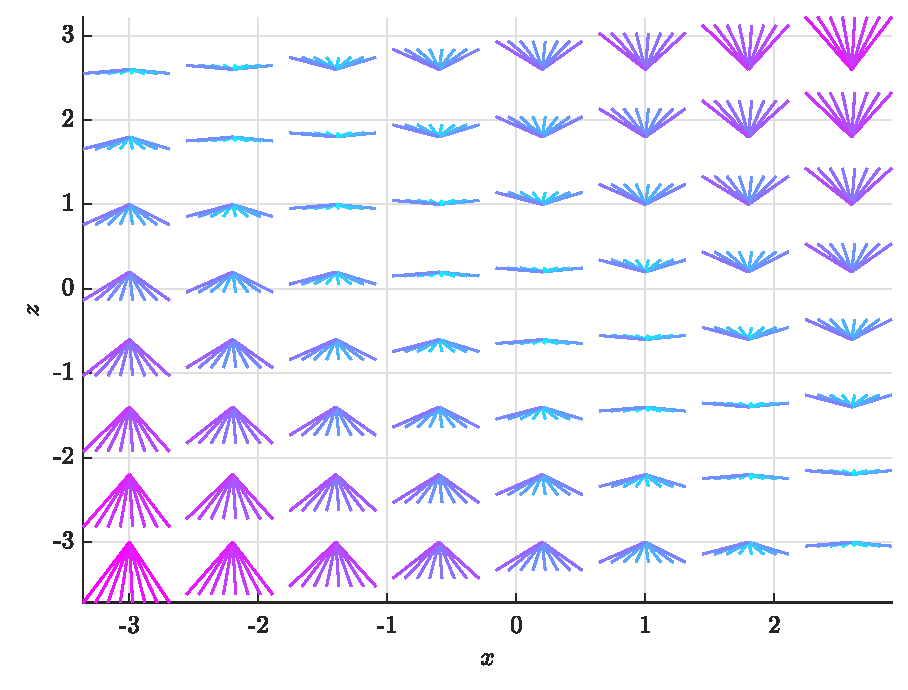
\includegraphics[width=\textwidth]{figures/vecfield_xz}
        \caption{$\vecfieldV$ when looking towards the $xz$-plane.}
    \end{subfigure}
\end{figure}
\begin{enumerate}[(a)]
    \item \textbf{(2 pts.)} Does this vector field have divergence? Explain.
    \item \textbf{(2 pts.)} Does this vector field have curl? Explain.
\end{enumerate}
\end{problem}



\begin{problem}
\textbf{(2 pts.)}  Let $f$ be a scalar field with gradient $\grad f$. Suppose as well that $\grad f$ has no divergence. Explain or show why $\Delta f = 0$.
\end{problem}  

\end{document}  